\documentclass[11pt,a4paper]{article}
\usepackage[top=12mm,bottom=10mm,left=15mm,right=15mm]{geometry}
\usepackage{tikz}
\usepackage{amsmath,amssymb}
\usepackage{booktabs}
\usepackage[T1]{fontenc}
\usepackage{lmodern}
\usepackage{microtype}
\usepackage{xcolor}
\usetikzlibrary{positioning,arrows.meta,fit,backgrounds,calc,shapes.geometric}
\usepackage{listings}
\pagestyle{empty}

\definecolor{ink}{HTML}{1A1A1A}
\definecolor{tensor}{HTML}{1F6F4A}
\definecolor{seq}{HTML}{1F4E8C}
\definecolor{prod}{HTML}{9C3B1B}
\definecolor{sum}{HTML}{6B4E9C}
\definecolor{pale}{HTML}{F4F2ED}
\definecolor{grey}{HTML}{6E6A63}

\lstset{basicstyle=\ttfamily\scriptsize, language=Java, keywordstyle=\color{ink},
        commentstyle=\color{grey}\itshape, showstringspaces=false, columns=fullflexible}

\tikzset{
  srv/.style={draw=ink, fill=white, rounded corners=2pt, inner sep=4pt,
              font=\footnotesize\ttfamily, minimum height=7mm, minimum width=20mm},
  plan/.style={srv, fill=pale, font=\footnotesize\ttfamily\bfseries},
  op/.style={circle, draw, inner sep=1pt, minimum size=7mm, font=\small\bfseries},
  ar/.style={-{Stealth[length=2mm]}, thick, color=grey},
  lbl/.style={font=\scriptsize\itshape, color=grey},
}

\begin{document}

\begin{center}
{\LARGE\bfseries The four combinators, and where each one fires}\\[1.5mm]
{\small \texttt{stalin} --- \S5 of Ghani, \emph{Containers for Typed Agentic AI}}\\[0.5mm]
{\footnotesize\color{grey} A container is $(P,R)$: a type of prompts, and a
prompt-indexed type of valid replies.\\
Every box below is one. Every arrow is a prompt going down and a reply coming back.}
\end{center}

\vspace{1mm}

% ─────────────────────────── the flow chart ───────────────────────────
\begin{center}
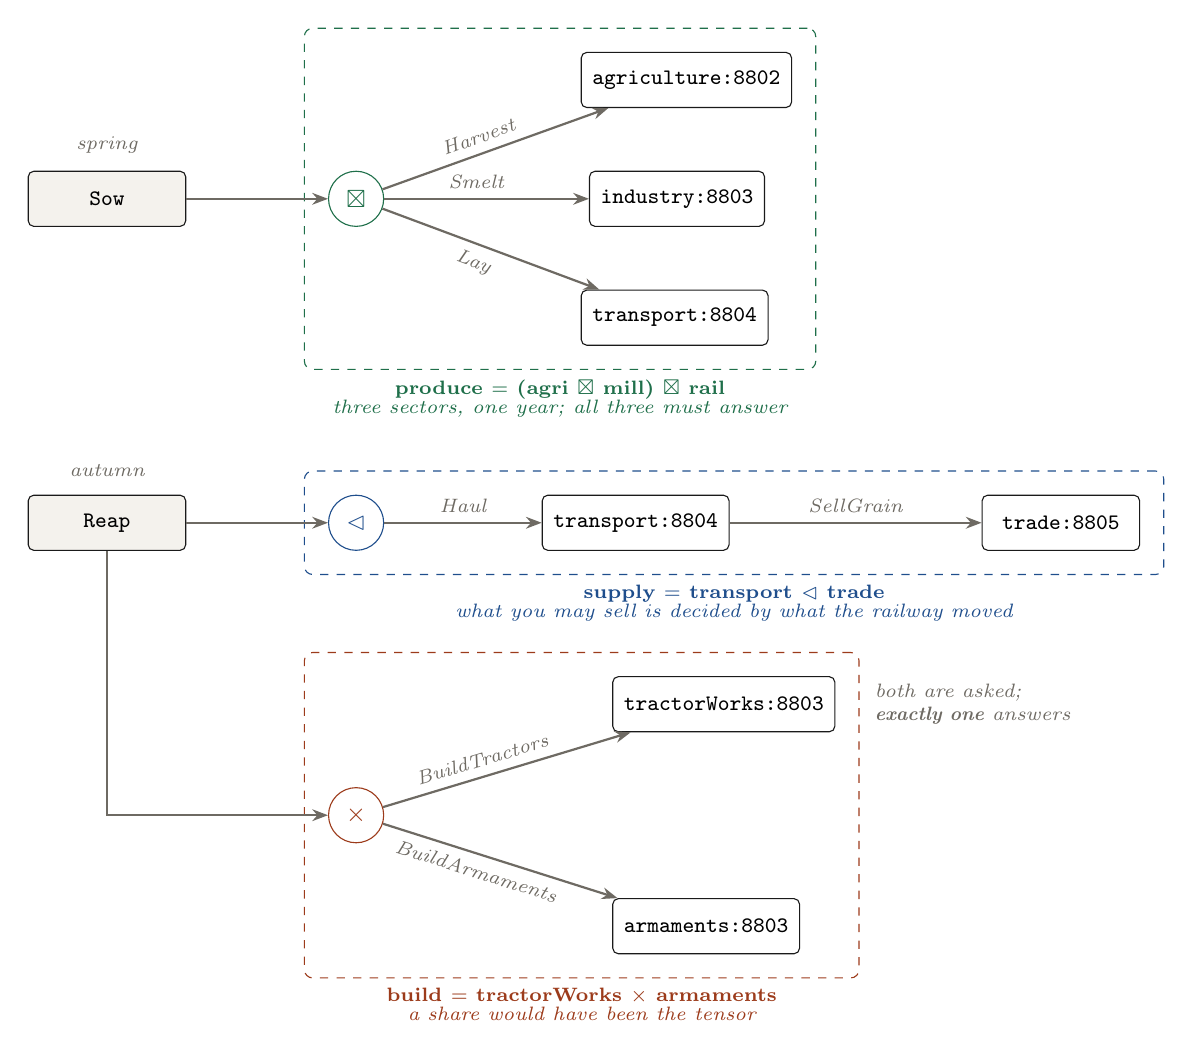
\begin{tikzpicture}[node distance=6mm]

% --- SPRING ---
\node[plan] (sow) {Sow};
\node[lbl, above=1mm of sow] {spring};

\node[op, draw=tensor, text=tensor] (t1) [right=18mm of sow] {$\boxtimes$};
\node[srv] (agri)  [above right=9mm and 26mm of t1] {agriculture:8802};
\node[srv] (mill)  [right=26mm of t1] {industry:8803};
\node[srv] (rail)  [below right=9mm and 26mm of t1] {transport:8804};

\draw[ar] (sow) -- (t1);
\draw[ar] (t1) -- node[lbl, pos=0.45, above, sloped] {Harvest} (agri);
\draw[ar] (t1) -- node[lbl, pos=0.45, above] {Smelt} (mill);
\draw[ar] (t1) -- node[lbl, pos=0.45, below, sloped] {Lay} (rail);

\begin{scope}[on background layer]
\node[fit=(t1)(agri)(mill)(rail), draw=tensor, dashed, rounded corners=3pt,
      inner sep=3mm, label={[font=\scriptsize\bfseries, text=tensor, align=center]below:%
      produce $=$ (agri $\boxtimes$ mill) $\boxtimes$ rail\\[-0.4mm]
      {\normalfont\itshape\scriptsize three sectors, one year; all three must answer}}] {};
\end{scope}

% --- AUTUMN ---
\node[plan] (reap) [below=34mm of sow] {Reap};
\node[lbl, above=1mm of reap] {autumn};

\node[op, draw=seq, text=seq] (s1) [right=18mm of reap] {$\lhd$};
\node[srv] (rail2) [right=20mm of s1] {transport:8804};
\node[srv] (trade) [right=32mm of rail2] {trade:8805};

\draw[ar] (reap) -- (s1);
\draw[ar] (s1) -- node[lbl, pos=0.5, above] {Haul} (rail2);
\draw[ar] (rail2) -- node[lbl, pos=0.5, above] {SellGrain} (trade);

\begin{scope}[on background layer]
\node[fit=(s1)(rail2)(trade), draw=seq, dashed, rounded corners=3pt,
      inner sep=3mm, label={[font=\scriptsize\bfseries, text=seq, align=center]below:%
      supply $=$ transport $\lhd$ trade\\[-0.4mm]
      {\normalfont\itshape\scriptsize what you may sell is decided by what the railway moved}}] {};
\end{scope}

% --- PRODUCT ---
\node[op, draw=prod, text=prod] (p1) [below=30mm of s1] {$\times$};
\node[srv] (tract) [above right=8mm and 30mm of p1] {tractorWorks:8803};
\node[srv] (arms)  [below right=8mm and 30mm of p1] {armaments:8803};

\draw[ar] (reap) |- (p1);
\draw[ar] (p1) -- node[lbl, pos=0.42, above, sloped] {BuildTractors} (tract);
\draw[ar] (p1) -- node[lbl, pos=0.42, below, sloped] {BuildArmaments} (arms);
\node[lbl, right=4mm of tract, align=left, text width=34mm]
  {both are asked;\\\textbf{exactly one} answers};

\begin{scope}[on background layer]
\node[fit=(p1)(tract)(arms), draw=prod, dashed, rounded corners=3pt,
      inner sep=3mm, label={[font=\scriptsize\bfseries, text=prod, align=center]below:%
      build $=$ tractorWorks $\times$ armaments\\[-0.4mm]
      {\normalfont\itshape\scriptsize a share would have been the tensor}}] {};
\end{scope}

\end{tikzpicture}
\end{center}

\vspace{2mm}

% ─────────────────────────── the table ───────────────────────────
\begin{center}
\footnotesize
\begin{tabular}{@{}c l l@{}}
\toprule
& \textbf{what it means} & \textbf{where it fires in \texttt{stalin}} \\
\midrule
\textcolor{tensor}{$\boxtimes$} & shapes multiply, positions multiply:
  & the three sectors work the \emph{same} year. \\
 & ask both, and both must answer
  & both shapes are supplied \emph{up front}, so\\
 & & neither can depend on the other's reply. \\[1.5mm]
\textcolor{seq}{$\lhd$} & the shape is a dependent pair
  & what can be \emph{sold} depends on what the \\
 & $(s : A \mathbin{**} A.\mathrm{Pos}\,s \to B)$: a first prompt
  & railway actually \emph{moved}. The second prompt \\
 & \emph{together with} a function choosing
  & is not knowable when the first is sent. \\
 & the second from the first's reply & \\[1.5mm]
\textcolor{prod}{$\times$} & offer both, owe exactly one
  & this year's steel becomes tractors \emph{or} \\
 & --- $\mathrm{Either}\,(R\,p)\,(T\,q)$
  & armaments. A \emph{share} would have been the \\
 & & tensor; calling that a product would be false. \\[1.5mm]
\textcolor{sum}{$+$} & routing: a coproduct of shapes,
  & \textbf{never built as a composite.} It appears as
  \\
 & eliminated by case analysis
  & each container's own shape type --- a tagged \\
 & & union --- and its eliminator is the
  \texttt{switch} \\
 & & in every server's dispatch. Real work, in the \\
 & & place \S3 always put it; but no \texttt{sumC(...)} call, \\
 & & and it would be an overstatement to claim one. \\
\bottomrule
\end{tabular}
\end{center}

\vspace{1.5mm}
\noindent\begin{minipage}[t]{0.485\textwidth}
\scriptsize\color{grey}
\textbf{Two that used to be here.} While the line to the port was narrow the
sale was a \emph{product} (grain \emph{or} steel, one contract) and became a
\emph{tensor} once enough rail was laid --- rail capacity choosing between
$\times$ and $\boxtimes$. Selling steel was removed from the game, so both
would have been running on a quantity that is permanently zero. They were
deleted rather than left for a diagram to claim.
\end{minipage}\hfill
\begin{minipage}[t]{0.485\textwidth}
\scriptsize\color{grey}
\textbf{One that broke and was repaired.} Splitting the year put
\texttt{produce} in spring and the haul in autumn, with a player decision
between them, so \texttt{seqC(produce, transport)} could no longer run in a
single call --- it stayed declared and silently never fired. The dependent pair
had not disappeared; it had moved one link down the chain. Hence
\texttt{seqC(transport, trade)}: haul, \emph{then} sell what reached the port.
\end{minipage}

\end{document}
